\documentclass[11pt]{aucklandthesis}
%
% This is a template for University of Auckland theses.
%
% Written by Alistair Kwan, June 2016
% 
%
% Options:
%	10pt, 11pt, 12pt: size of main text
% 	examcopy: asserts confidentiality for examination copies
%	partial: thesis partial fulfils degree requirements
%	singlespace, onehalfspace, doublespace: line spacing
%	oneside: format for single-sided printing
%	draft: adds 'draft' and date to footer
%

%
% Add, delete or un-comment packages below as required.
%

\usepackage[utf8]{inputenc}
\usepackage[T1]{fontenc}

%\usepackage{graphicx} % for inserting graphics files
%\usepackage{appendix} % for appendices

%\usepackage{hyperref} % for formatting web addresses and other URLs
%\urlstyle{same} % try also tt, sf if this option doesn't produce clear enough output

% Readability options
%
%\usepackage{booktabs} % for table rules
%\usepackage{microtype} % for improved justification

% Typeface options — choose one if desired
% or choose a different typeface to accommmodate character sets
% as needed for East Asian and other languages.
%
% Consider compiling using the XeLaTeX engine if you have more extreme
% typeface needs, e.g. for multiple languages, or a need for symbols particular
% to a typeface.
%
% See also the LaTeX Symbols List at
% https://http://www.ctan.org/pkg/comprehensive
%
%\usepackage{mathptmx} % Times New Roman, including mathematics
%\usepackage{mathpazo} % Palatino with mathematics support
%\usepackage{fourier} % Utopia, a serif typeface with Fourier mathematics
%\usepackage{gentium} % a contemporary serif typeface
%\usepackage{libertine} % a softer-feeling serif typeface; also installs sans-serif font Biolinum
%\usepackage{fouriernc} % Century Schoolbook with Fourier maths
%\usepackage{mathpple} % Palatino with Fourier maths


% To set the sans serif font (for \sffamily):
%\usepackage[scaled]{helvet} % Nimbus, like Helvetica
%\usepackage{universalis} % Universalis
%\usepackage{avant} % URW Gothic, like Avant Garde
%\usepackage{PTSansNarrow}
%\usepackage{AlegreyaSans} % Alegreya Sans

% To set the mathematics font:
%\usepackage{eulervm} % Euler, based on a Zapf design

% To set the (usually monospaced) typewriter font:
%\usepackage[ttdefault=true]{AnonymousPro}
%\usepackage[scaled]{beramono}
%\usepackage{inconsolata}
%\usepackage{sourcecodepro}

%\usepackage{cjk} % for Chinese, Japanese, Korean

%\usepackage{tabularx} % For easier table formatting.

%\usepackage[nottoc]{tocbibind} % Controls the table of contents
%   nottoc: don't list table of contents inside itself
%   section: go as far as section-level headings

% Automated bibliography
%
%\usepackage[
%	style=authortitle, 
%	citestyle=authortitle,
%	backend=biber
%	]
%	{biblatex}
%bibliography{bibliography1.bib, bibliography2.bib} % Specify bibliography files 

\begin{document}

% ====================================================
%
% FRONTMATTER
%
% Arabic pagination, starting with the title page
% which is counted but not numbered
%
% ====================================================

% Specify the title page content
\title{[thesis title]}
\subtitle{[subtitle]}
\author{[candidate's name]}
\degreesought{[degree]} 
\degreediscipline{[discipline]}
\degreecompletionyear{[year]}

% Print the title page
\maketitle

% Abstract, up to 350 words
%% !TEX root = main.tex
% !TEX encoding = Windows Latin 1
% !TEX TS-program = pdflatex
% 
% Archivo: abstract.tex (en ingles)


\chapter{Abstract} % No cambiar el titulo
\selectlanguage{english}
\noindent
Duis tristique sollicitudin leo nec consequat. Praesent et dui convallis velit tincidunt fermentum. Mauris cursus purus at sem viverra sed imperdiet sapien imperdiet. Aliquam mattis, elit eget rutrum vulputate, tortor sem pulvinar justo, sit amet mollis felis sem at nibh. Donec malesuada, neque id interdum eleifend, arcu augue porta elit, nec tristique libero metus at massa. Fusce fringilla laoreet rhoncus. Suspendisse potenti. Phasellus dignissim sodales mauris at pharetra. Donec gravida fringilla velit ac rutrum.

Curabitur ornare lectus id diam molestie eu imperdiet nulla tempus. Maecenas vestibulum enim et dui ornare blandit. Vivamus fermentum faucibus viverra. Maecenas at justo sapien. Aenean rhoncus augue mattis purus rhoncus venenatis. Suspendisse metus felis, porttitor in varius in, vulputate at tortor. Aliquam molestie, turpis et malesuada porta, tortor sapien pharetra sapien, ac rhoncus quam dolor a sapien. Pellentesque varius laoreet enim ut auctor. Nullam nec ultricies nisi. Nullam porta lectus et ante consectetur posuere.

Duis tristique sollicitudin leo nec consequat. Praesent et dui convallis velit tincidunt fermentum. Mauris cursus purus at sem viverra sed imperdiet sapien imperdiet. Aliquam mattis, elit eget rutrum vulputate, tortor sem pulvinar justo, sit amet mollis felis sem at nibh. Donec malesuada, neque id interdum eleifend, arcu augue porta elit, nec tristique libero metus at massa. Fusce fringilla laoreet rhoncus. Suspendisse potenti. Phasellus dignissim sodales mauris at pharetra. Donec gravida fringilla velit ac rutrum.

Duis tristique sollicitudin leo nec consequat. Praesent et dui convallis velit tincidunt fermentum. Mauris cursus purus at sem viverra sed imperdiet sapien imperdiet. Aliquam mattis, elit eget rutrum vulputate, tortor sem pulvinar justo, sit amet mollis felis sem at nibh. Donec malesuada, neque id interdum eleifend, arcu augue porta elit, nec tristique libero metus at massa. Fusce fringilla laoreet rhoncus. Suspendisse potenti. Phasellus dignissim sodales mauris at pharetra. Donec gravida fringilla velit ac rutrum.

Curabitur ornare lectus id diam molestie eu imperdiet nulla tempus. Maecenas vestibulum enim et dui ornare blandit. Vivamus fermentum faucibus viverra. Maecenas at justo sapien. Aenean rhoncus augue mattis purus rhoncus venenatis. Suspendisse metus felis, porttitor in varius in, vulputate at tortor. Aliquam molestie, turpis et malesuada porta, tortor sapien pharetra sapien, ac rhoncus quam dolor a sapien. Pellentesque varius laoreet enim ut auctor. Nullam nec ultricies nisi. Nullam porta lectus et ante consectetur posuere.

Duis tristique sollicitudin leo nec consequat. Praesent et dui convallis velit tincidunt fermentum. Mauris cursus purus at sem viverra sed imperdiet sapien imperdiet. Aliquam mattis, elit eget rutrum vulputate, tortor sem pulvinar justo, sit amet mollis felis sem at nibh. Donec malesuada, neque id interdum eleifend, arcu augue porta elit, nec tristique libero metus at massa. Fusce fringilla laoreet rhoncus. Suspendisse potenti. Phasellus dignissim sodales mauris at pharetra. Donec gravida fringilla velit ac rutrum.

\bigskip
\noindent
\textit{Key words:} first word; second word; third word.
% Separar palabras con punto-y-comas.

\checklanguage
% Fin archivo abstract.tex
\endinput  % it's in a separate file

% Dedication (optional)
%\thesisdedication{Dedicated to grandma, and to grammar.}

% Preface and/or acknowledgements (optional)
%% !Mode:: "TeX:UTF-8"

历时将近两个月的时间终于将这篇论文写完,在论文的写作过程中遇到了无数的困难和障碍,都在同学和老师的帮助下度过了。尤其要强烈感谢我的论文指导老师—XX老师,她对我进行了无私的指导和帮助,不厌其烦的帮助进行论文的修改和改进。另外,在校图书馆查找资料的时候,图书馆的老师也给我提供了很多方面的支持与帮助。在此向帮助和指导过我的各位老师表示最中心的感谢!

感谢这篇论文所涉及到的各位学者。本文引用了数位学者的研究文献,如果没有各位学者的研究成果的帮助和启发,我将很难完成本篇论文的写作。

感谢我的同学和朋友,在我写论文的过程中给予我了很多你问素材,还在论文的撰写和排版灯过程中提供热情的帮助。
由于我的学术水平有限,所写论文难免有不足之处,恳请各位老师和学友批评和指正!
 % it's in a separate file

% Contents, lists of tables and figures
\settocdepth{section} % choose chapter, section, subsection \cleardoublepage\tableofcontents
%\cleardoublepage\listoffigures
%\cleardoublepage\listoftables

% Glossary (optional)
%\input{glossary}

% ====================================================
%
% MAINMATTER
%
% Include external chapter files here using
% the \input{} command
%
% If you run out of memory during compilation,
% switch some or all chapters to \include{} instead of \input{}, 
% but watch out for pagination problems.
%
% ====================================================

%%
% Modified by Sameer Vijay
% Last Change: Tue Jul 26 2005 13:00 CEST
%
%%%%%%%%%%%%%%%%%%%%%%%%%%%%%%%%%%%%%%%%%%%%%%%%%%%%%%%%%%%%%%%%%%%%%%%%
%
% Sample Notre Dame Thesis/Dissertation
% Using Donald Peterson's ndthesis classfile
%
% Written by Jeff Squyres and Don Peterson
%
% Provided by the Information Technology Committee of
%   the Graduate Student Union
%   http://www.gsu.nd.edu/
%
% Nothing in this document is serious except the format.  :-)
%
% If you have any suggestions, comments, questions, please send e-mail
% to: ndthesis@gsu.nd.edu
%
%%%%%%%%%%%%%%%%%%%%%%%%%%%%%%%%%%%%%%%%%%%%%%%%%%%%%%%%%%%%%%%%%%%%%%%%


%
% Chapter 1
%

\chapter{INTRODUCTION}

\section{Overview}

This is an overview of the introduction.  In here, I will use many
many buzzwords and other legalistic-types of terms, mostly begining on
the expounding of the holistic and synergistic energy that Gnus bring
to our organizations.

\subsection{Background}

In preparation for reading this dissertation, I would highly recommend
reading some of the other material available on
Gnus~\citep{gnus98:_gerry_ganst,greenfield96:_gettin_know_gnu}.  They
are very well written and will give you a fuller understanding of
Gnus.

Gnus are frequently mistakes for squirrels.  They are not squirrels.
They are Gnus.  Don't call them squirrels, either (unless you have
food in your hand); they tend to get a bit upset.\footnote{This is
  frequently mistaken for the chattering and scampering away.  Gnus
  are actually quite polite; they will leave if they have nothing nice
  to say, for fear of saying something offensive.}  If you have food
in your hand, they tend to ignore this insult and accept your food as
a peace offering.

\subsection{Foreground}

Table~\ref{tbl:bogus1} shows some feeding frequencies for where Gnus
like to eat around the Notre Dame campus.  Gnus have work weeks, just
like humans do, hence the much lower frequencies on weekends.  This
can lead us to conclude that Gnu weekend shifts are much smaller than
the normal work-week shifts.  In fact, we can attempt to parametrize the
sighting frequency, $\mathcal{F}$, by the student population, type of food, and
day of the week as:
\begin{equation}
  \mathcal{F} = \mathcal{F}(p,f,d).
\end{equation}
Table~\ref{tbl:bogus2} shows what they
typically like to eat.

\begin{table}[tpb]
  \begin{center}
    \caption{WHERE Gnus LIKE TO EAT \label{tbl:bogus1}}
    \begin{tabularx}{0.85\textwidth}{lrrrrrrr} \toprule
      \multicolumn{1}{c}{Location} & Sun & Mon & Tue & Wed & Thu & Fri & Sat \\ \midrule
      Front of Dome & 1 & 5 & 6 & 5 & 4 & 5 & 1 \\
      Stonehenge & 2 & 9 & 10 & 12 & 9 & 14 & 2 \\
      The Rock & 1 & 3 & 4 & 3 & 4 & 3 & 0 \\
      The ACC & 3 & 4 & 5 & 5 & 5 & 4 & 1 \\
      Dining Halls & 5 & 14 & 12 & 13 & 14 & 12 & 3 \\
      Hesburgh Library & 2 & 3 & 5 & 2 & 3 & 4 & 2 \\ \bottomrule
    \end{tabularx}
  \end{center}
\end{table}

\begin{table}[tpb]
  \setlength{\capwidth}{0.7\textwidth}
  \begin{center}
    \caption{WHAT Gnus LIKE TO EAT ON THE NOTRE DAME CAMPUS, LISTED
      BY AVERAGE NUMBER OF SIGHTINGS PER WEEKDAY
    \label{tbl:bogus2}
}
    \begin{tabular}{lrrrrrrr} \toprule
      \multicolumn{1}{c}{Food} & Sun & Mon & Tue & Wed & Thu & Fri & Sat \\ \midrule
      Twinkies & 1 & 5 & 6 & 5 & 4 & 5 & 1 \\
      Ding Dongs & 2 & 9 & 10 & 12 & 9 & 14 & 2 \\
      Carrots & 1 & 3 & 4 & 3 & 4 & 3 & 0 \\
      Lettuce & 3 & 4 & 5 & 5 & 5 & 4 & 1 \\
      Twizlers & 5 & 14 & 12 & 13 & 14 & 12 & 3 \\
      Jawbreakers & 2 & 3 & 5 & 2 & 3 & 4 & 2 \\ \bottomrule
    \end{tabular}
  \end{center}
\end{table}

Figure~\ref{fig:bogus3} shows a nice graph of location distributions
by day of week.  I have no real reason for including it except to show
that figures work as well.  Did I mention that Gnus are really cool?

\begin{figure}[tpb]
  \begin{center}
    \centerline{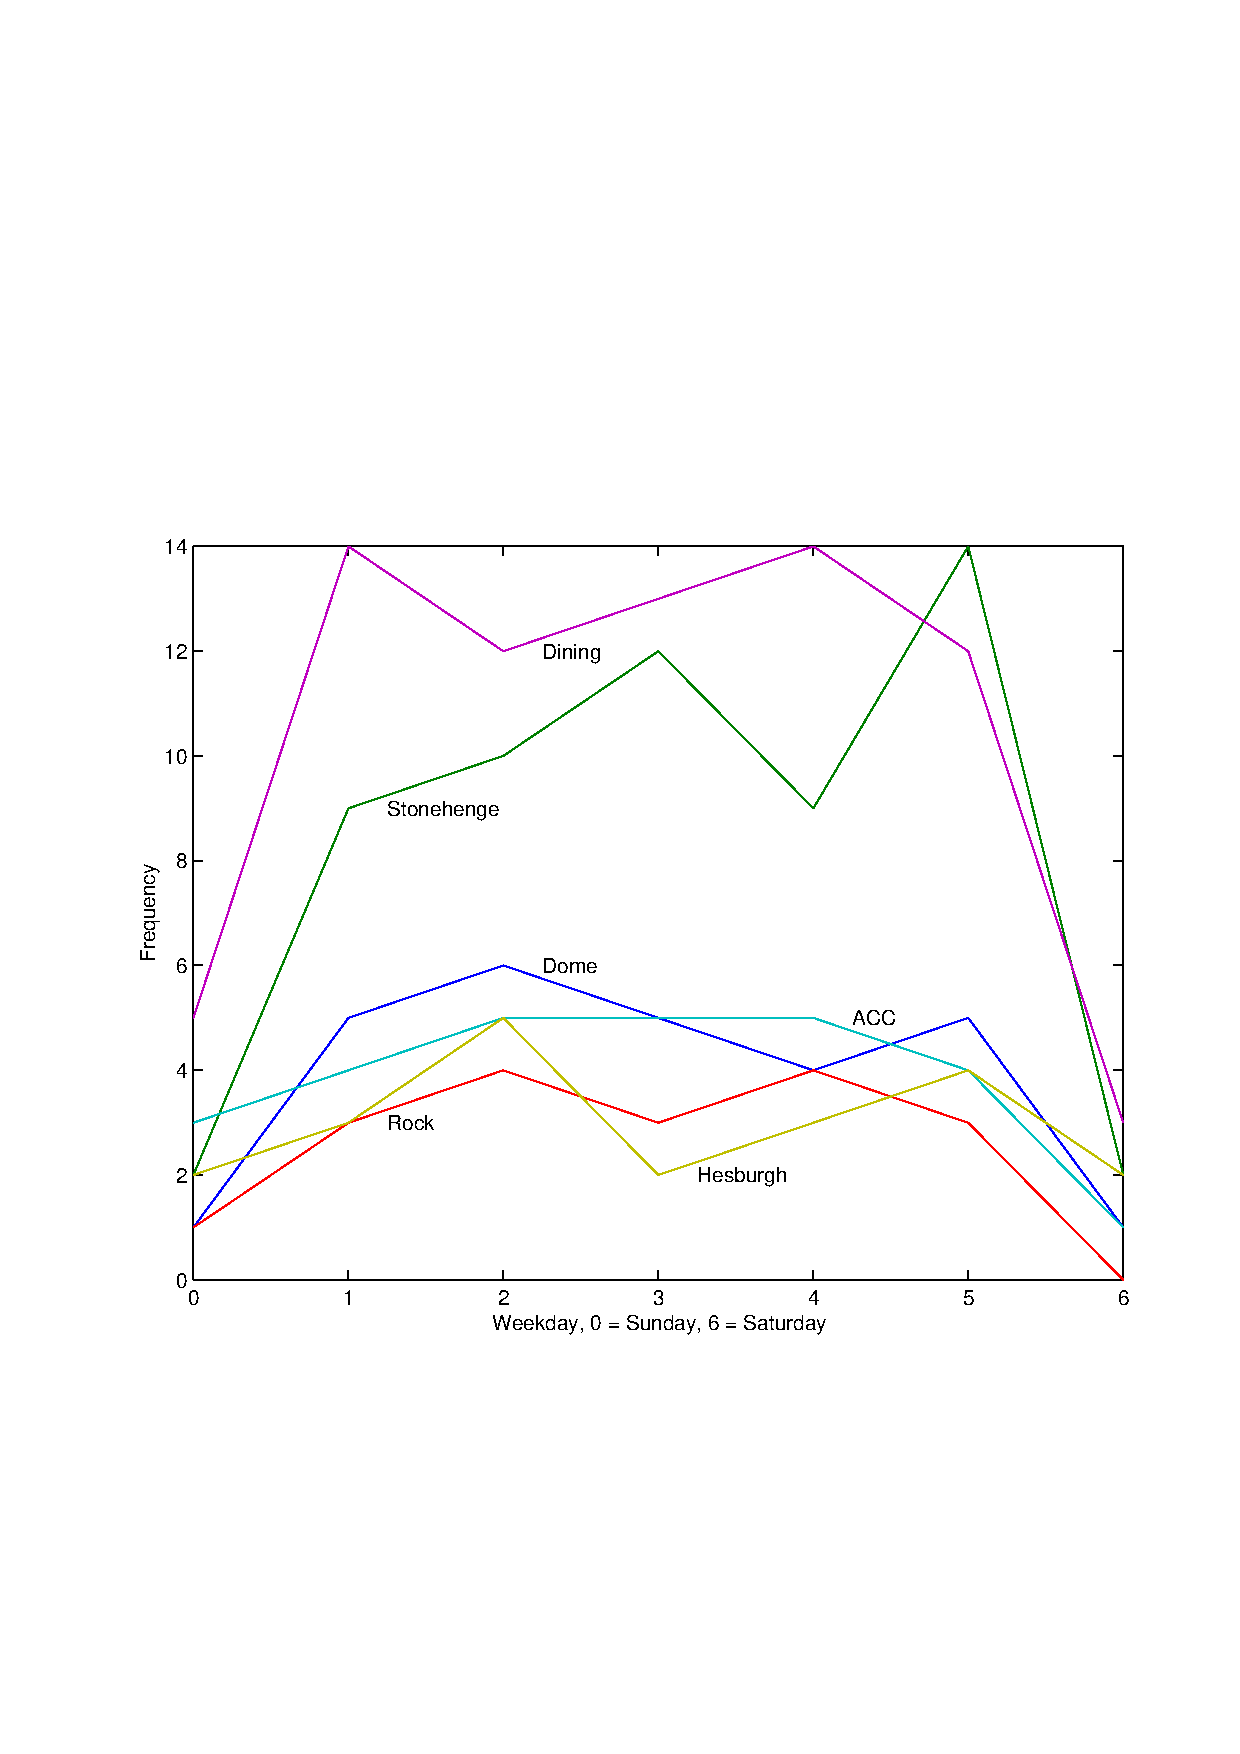
\includegraphics[scale=0.8]{sample_nd}}
    \caption{Location distributions by day of where, where the X axis
      is the weekday (0 through 6), and the Y axis is the sighting
      frequency}
    \label{fig:bogus3}
  \end{center}
\end{figure}

Gnus typically tend to come out when there are large gatherings of
humans with food.  Gnus work very hard at providing us with all the
things that we like (trees, dirt, air, etc.), and so we should freely
give them food.  They will come up and stand a respectful distance
away from you, waiting to see if they will be rewarded for their
efforts.  If you offer some food, they will take it and back off a
respectful distance in order to consume their food while leaving you
to your ``personal space.''  

\section{Groovin' Gnus}
\label{sec:groovin-gnus}

Gnus do tend to stay away from humans in their normal day-to-day
workings.  This is mainly because humans don't, for the most part,
understand what they are doing.  If a Gnu is working, and a human
approaches it, the Gnu will tend to drop whatever it is doing and run
away.  This is probably do to the tendency for humans to have ``group
meetings'' and ``productivity seminars.''  Most Gnus are deathly
afraid of such overmanagement, and run at the slightest hint of it,
for fear that it will cripple their real work.

It is interesting, however, that Gnus have chosen an Institution of
Higher Education for their BOO.\footnote{Base of Operations.}  It is
often said that:
\begin{quote}
  Academic politics are the dirtiest, meanest, ugliest, and generally
  the most low-down, in-your-face, and kick-em-while-they're-down than
  anywhere else (even Washington D.C.)  because the stakes are so low.
\end{quote}
It has been hypothesized that the Gnus are subtly trying to affect a
change for the better (i.e., eliminating the overmanagement problems)
by working the very system that they are trying to change, from
within.  That is, the graduates from Notre Dame can learn from the
examples of the Gnus here, and run screaming (or chattering) at the
slightest hint of overmanagement, and let the real work proceed
unhindered.

% % uncomment the following lines,
% if using chapter-wise bibliography
%
% \bibliographystyle{ndnatbib}
% \bibliography{example}
 % I hope that you have better titles than this
%\chapter{فضاهای فشرده پایدار و فضاهای مرتب فشرده}
\thispagestyle{empty}
\section{فضاهای فشرده پایدار}
یک فضای توپولوژیک جزئاً مرتب (یا به طور خلاصه، فضای مرتب)، از دیدگاه آبرامسکی
\cite{abramsky2}،
مجموعه‌ای مانند $ X $ همراه 
با یک توپولوژی $ \mathcal{O} $ و یک ترتیب $ \leq $ است به طوری که گراف ترتیب در $X\times X  $ بسته باشد. بنابراین ...
\section{فضاهای مرتب فشرده}
در این  بخش به بیان ... 
%\chapter{اندازه‌ها و ارزیابی‌ها}
\thispagestyle{empty}
\section{اندازه‌ها و تابعی‌های خطی مثبت روی $\mathrm{C(X)}$}
فرض کنید $X$ یک فضای توپولوژیکی روی ...
\section{تابعی‌های خطی}
در این بخش ... 

% ====================================================
%
% ENDMATTER
%
% Appendices and bibliography 
% Pagination arabic, re-starts at 1
%
% ====================================================
\cleardoublepage % start afresh on a new page
\setcounter{page}{1} % re-sets the page counter
%\appendixpage* % makes a page to mark beginning of appendices
% \chapter{Test Appendix with a very long title in order to test spacing behavior} \label{app:test}
\lipsum[2]

A convenient form for representing substantial numerical or textual data is a table. 
Table~\ref{tab:test} shows an example of this functionality in \LaTeX.
\begin{table}
  \centering
  \caption{Test table. With an extra-long caption to test spacing functionality for table captions. And inline mathematics.}
  \begin{tabular}{lrr}
    \toprule
    Heading 1 ($u_x$)  & Head 2 & Head 3 \\
    \midrule
    Analytical         & 1.000  & 1.000  \\
    Forward Difference & 0.973  & 0.976  \\
    \bottomrule
  \end{tabular}
  \label{tab:test}
\end{table}
Diagrams, plots, and other graphics should be placed in figures. 
Figure~\ref{fig:test} shows an example of such an environment.
The command \verb+\includegraphics+ from the \verb+graphicx+ package may be used to include external graphics in a wide variety of formats.
\begin{figure}
  \centering 
  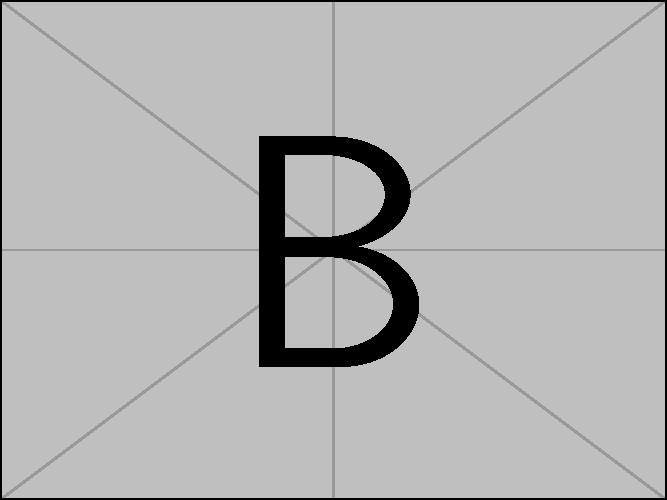
\includegraphics[width=1in]{example-image-b}
  \caption{This test figure tests captions and Table of Contents 
    behavior for lengthy captions.}
  \label{fig:test}
\end{figure}

\section{This is a Very Long Heading to Test the Table of Contents Behavior for Very Long Section Headings}
Sample text. Sample text.

\subsection{This is an Extremely Long Subsection Heading to Test Spacing Behavior for Subsections}
\lipsum[3]

\subsubsection{This is an Extremely Long Subsubsection Heading to Test Spacing Behavior for Subsubsections}
\lipsum[4-5]
 

%\printbibliography[title={Works cited}, heading=bibintoc]

\end{document}